\documentclass[aps,pra,twocolumn]{revtex4-1}

\usepackage{graphicx,epstopdf}
\usepackage{amsmath}
\usepackage{mathtools}
\usepackage{mathrsfs}


\begin{document}


\title{On the dynamics of gravitational stability in protoplanetary disks}

\author{Evan Anders}
\affiliation{Department of Physics, Whitworth University, 300 W. Hawthorne Rd., Spokane, WA 99251}


\date{\today}

\begin{abstract}
Protoplanetary disks are astrophysical objects which surround young stars and are generally modeled as geometrically thin cylinders.  Here we examine the basic dynamics of such disks, including the effects of the gravitational and centripetal forces on the disks, as well as the effects of viscosity and random motions of particles.  We observe the effects of such parameters on disk stability, and briefly outline the regimes under which such instabilities can form distinct bound objects.
\end{abstract}



\maketitle


\section{\label{section1} Introduction}

Protoplanetary disks are an observed phenomena which surround young stars and display early conditions of planet formation.  These disks typically persist with lifetimes on the order of $10^6$ years and have masses far lower than the stellar mass and are distinctly different from debris disks which surround older stars.  As a result, it is exceptionally rare for observations of the evolution of these disks to be made.  Rather, their evolution must be described using statistical studies of populations and computational simulations.  Angular momentum conservation is at the heart of this slow evolution.   \cite{armitage2011}

A large body of the work that has been published on such protoplanetary disks pertains to basic topics of classical mechanics.  While there are a number of other, more complex phenomenon involved in disk evolution, such as magnetorotational instability and convection, gravitation--and gravitational instability--have offered insight on disk evolution and have informed a large portion of the literature throughout the past two decades.  In certain regimes, it is possible to model the disk using primarily base principles of classical mechanics and find that planetary formation can occur.  It is with such cases that this paper is focused on.  We will develop a schema for describing a rotating disk of particles primarily influenced by gravitational and centripetal forces.  We will apply base principles to such a disk in order to understand what gravitational instability truly means, and then we will discuss the results of gravitational instabilities in simulations from the current literature.  In the end, further topics which were not considered will be briefly discussed.



\section{\label{section 2} A schema for the description of disk evolution}
\begin{figure} [b!]
	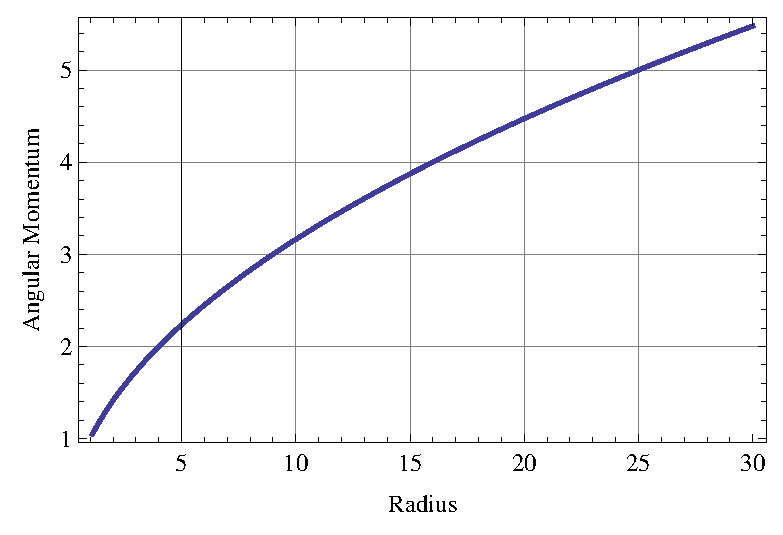
\includegraphics[width=3in]{angularMomentum.eps}
	\caption{This plot shows a the trend that angular momentum follows in protoplanetary disks, as described in Eq. (\ref{angMomEq}).  This plot was created for nonspecific values of variables and constants, i.e. $m_p = G = M_* = 1$. \label{angMom}}
\end{figure}


Protoplanetary disks are modeled as thin cylinders in cylindrical polar coordinates $(r, \phi, h)$.  The thin nature of such disks provides for us the assumption that $h_{\text{max}} \ll r_{\text{max}}$.  The thinness of the disk, along with the fact that it is fluid in nature, being primary constituted out of gas and dust, allows us to assume that the mass of the disk is significantly lower than that of the star, or $M_{\text{disk}} \ll M_{*}$.  

Taking all of these assumptions into account, we model each gas or dust particle at radius $r$ as having some mass, $m_p$.  We know that these particles are influenced by what is essentially a gravitational point mass at the location of the star \cite{armitage2011}.  For such a particle, we obtain the equation of motion \cite{taylor2005},
\begin{equation}
m_p \vec{a}_r = m_p ( \ddot{r} - r\dot{\phi}^2 )\hat{r} = - \frac{G M_* m_p}{r^2}\hat{r} . \label{rMotion}
\end{equation}
Assuming that the disk is not collapsing in upon itself or rapidly expanding outward, we can model it as a thin accretion disk.  Solving Eq. (\ref{rMotion}) for the Keplerian angular velocity under the assumption that $\ddot{r} = 0$, we find \cite{armitage2011}
\begin{equation}
\dot{\phi} = \Omega_K = \sqrt{\frac{G M_*}{r^3}}.
\end{equation}
As a result, the angular momenta of the disk particles can be expressed such that \cite{taylor2005},
\begin{equation}
\ell = \left| \vec{r} \times \vec{p} \right| = m_p r^2 \Omega_K = m_p \sqrt{G M_* r}, \label{angMomEq}
\end{equation}
which clearly increases as $\sqrt{r}$, as shown in Fig. \ref{angMom}.  

As we assumed that our disk is an accretion disk, we must account for angular momentum must be lost among the disk constituents.  There are two possible mechanisms for this loss of angular momentum: (i) the momentum is redistributed within the disk or (ii) the momentum is lost to an external sink \cite{armitage2011}.  This paper is primarily focused upon the former, with respect to how the gravity of the star and neighboring particles affect the motion of disk constituents.


\subsection{\label{section2.1} A model of evolution in accretion disks }
Among thin disks as described in the previous section, the vertical structure of the disk becomes insignificant.  As such, we integrate over this thickness in order to obtain a surface mass density, $\mu(r, t)$  \cite{armitage2011}.  Additionally, under the assumption of accretion, we know that in addition to the primary azimuthal velocity,
\begin{equation}
u_\phi = r\Omega_K
\end{equation}
disk particles have some radial `drift' velocity, $u_r$.  This drift velocity is negative close to the star, depends upon both $r$ and $t$, and is characterized by the surface density $\mu$.  In order to understand the evolution behavior of the disk, we must examine an infinitesimally thin ring between some radii, $R$ and $R + dr$.  This thin ring has a total mass of $M_\text{ring} = \pi \left(2 R dr + dr^2 \right)\mu \approx (2 \pi R \mu) dr$ and, therefore, a total angular momentum of $\ell_\text{ring} = (2\pi R^3 \mu \Omega_K)dr$ \cite{king2002}.

\subsubsection{\label{section 2.1.1} Conservation of mass}
By conservation of mass, we know that any change in the mass of our thin ring is a direct result of mass flowing in from neighboring sections of the disk, both radially inward and radially outward.  Thus,
\begin{equation}
\begin{split}
\frac{\partial}{\partial t}\left(  M_\text{ring}\right)= M_{\text{in}}(R) + M_{\text{in}}&(R + dR)  \\
= 2\pi [ R u_r(R, t) \mu&(R, t) -   \\
(R + dR)& u_r(R+dR, t) \mu(R+dR, t)] \\
 \approx -2\pi dR \frac{\partial}{\partial r}(R\mu& u_r),
\nonumber
\end{split}
\end{equation}
which provides for us the mass conservation equation in the limit $dr \rightarrow 0$ where,
\begin{equation}
\frac{\partial}{\partial t}\left(  2\pi R  \mu dr \right) + 2\pi dr \frac{\partial}{\partial r}(R \mu u_r) = 0. \nonumber
\end{equation}
Generalizing from our specific case at $R$ to any $r$ within the disk, our equation for conservation of mass is \cite{king2002},
\begin{equation}
r \frac{\partial \mu}{\partial t} + \frac{\partial}{\partial r}(r \mu u_r) = 0. \label{consMass}
\end{equation}

\subsubsection{\label{section 2.1.2} Conservation of angular momentum}
We approach conservation of angular momentum in manner similar to that which we used to determine the governing equation for conservation of mass. In addition to accounting for the flow of mass in an out of our thin ring, we must also add on a term which relates to the change caused by viscous torques, $\Gamma(r, t)$, and we find that
\begin{equation}
\frac{\partial}{\partial t}\left( \ell_{\text{ring}} \right) \approx  -2\pi dr \frac{\partial}{\partial r}(R^3 \mu u_r \Omega_K) + \frac{\partial \Gamma}{\partial r}dr.
\nonumber
\end{equation}
By isolating common terms and taking the limit as $dR \rightarrow 0$, we find our equation for conservation of angular momentum \cite{king2002},
\begin{equation}
R \frac{\partial}{\partial t} (\mu R^2 \Omega_K) + \frac{\partial}{\partial r} (R \mu u_r R^2  )\Omega_K' = \frac{1}{2\pi} \frac{\partial \Gamma}{\partial R}, \label{consAng}
\end{equation}
where
\begin{equation}
\Omega_K' = \frac{\partial \Omega_K}{\partial r}.
\end{equation}

\subsubsection{\label{section 2.1.3} Governing equation for surface density time evolution}
Using our equation for conservation of mass and assuming that $\Omega_K' = 0$, we can simplify our expression of conservation of angular momentum such that
\begin{equation}
R\mu u_r \frac{\partial}{\partial r} (R^2 \Omega_D) = \frac{1}{2\pi} \frac{\partial \Gamma}{\partial r}.
\end{equation}
Combining this equation with our equation for conservation of mass, we can eliminate $u_r$, such that
\begin{equation}
R \frac{\partial \mu}{\partial t} = -\frac{\partial}{\partial r}(R \mu u_r) = - \frac{\partial}{\partial r}\left[ \frac{1}{2\pi \frac{\partial}{\partial r}(R^2)\Omega_K'}\frac{\partial \Gamma}{\partial r} \right].
\end{equation}

For the case of an accretion disk with random particle motions, the flow of mass into and out of a region will create a change in angular momentum via a viscous torque.  Throughout the disk, we find that the torque per unit arc length follows the form \cite{king2002}
\begin{equation}
\gamma(r, t) = \nu \mu r^2 \Omega_K'.
\end{equation}
The total torque acting on any infinitely thin ring of radius $r$ takes on the form 
\begin{equation}
\Gamma(r, t) = 2 \pi r \gamma(r, t) = 2 \pi \nu \mu r^3 \Omega_K. \label{torque}
\end{equation}
we can solve for our equation of motion, which follows the form 
\begin{equation}
\frac{\partial \mu}{\partial t} = \frac{3}{r} \frac{\partial}{\partial r} \left| r^{1/2}\frac{\partial}{\partial r}\left( \nu \mu r^{1/2} \right) \right|
\end{equation}
as long as external torques and mass losses are neglected\cite{king2002, armitage2011}.  This follows directly from conservation of mass and angular momentum for a viscous fluid with kinematic viscosity $\nu$.


\subsection{\label{section 2.2} Characteristics of steady-state thin disks}
For a disk system in which external conditions change at timescales much longer than the radial structure of a thin disk, we can set time derivatives from our previous conservation equations, Eqs. (\ref{consMass}) and (\ref{consAng}) equal to zero.  In such a steady state, conservation of mass yields
\begin{equation}
R\mu u_r = constant, \nonumber
\end{equation}
from which it is easy to see that the total change of mass of the disk, or the accretion rate, takes on the form
\begin{equation}
\dot{M} = -2\pi R \mu u_r, \label{modifiedMass1}
\end{equation}
where the negative sign arises due to the fact that $u_r$ is in the inward radial direction.  Conservation of angular momentum yields
\begin{equation}
R^3 \mu u_r \Omega_K = \frac{\Gamma}{2\pi} + \frac{C}{2\pi} \nonumber
\end{equation}
for some constant $C$.  Plugging in the expression for torque found in Eq. (\ref{torque}) and rearranging, we find that \cite{king2002}
\begin{equation}
- \nu \mu \Omega_K' = -\mu u_r \Omega_K  + \frac{C}{2\pi R^3 }. \label{modifiedAng1}
\end{equation}


\subsubsection{\label{section 2.2.1} Relating mass flow, viscosity, and mass density}
\begin{figure} [b!]
	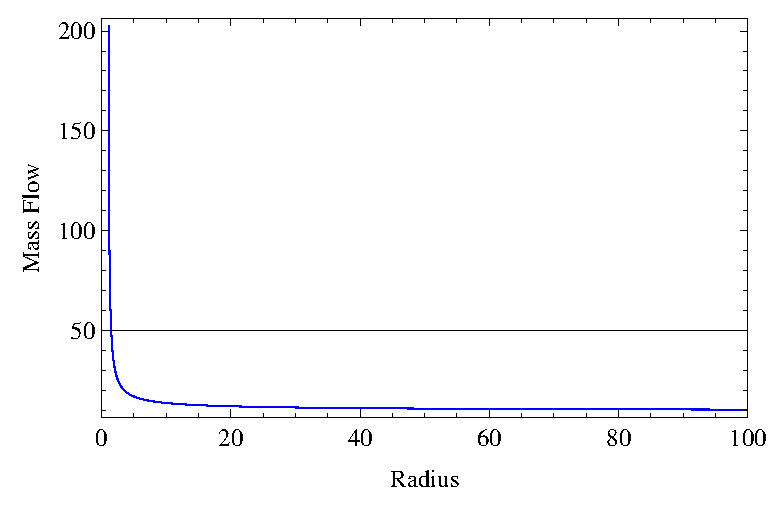
\includegraphics[width=3in]{massFlow.eps}
	\caption{This figure shows the shape of the relationship between mass flow rate and radius.  This plot was created using Eq. (\ref{massFlow}) with nonspecific values of other variables ($\nu = \mu = R_* = 1$).  Clearly, mass flow increases towards infinity as the star is approached, and at further radii it quickly drops off to a very low value. \label{massFlowFig}}
\end{figure}
\begin{figure} [t!]
	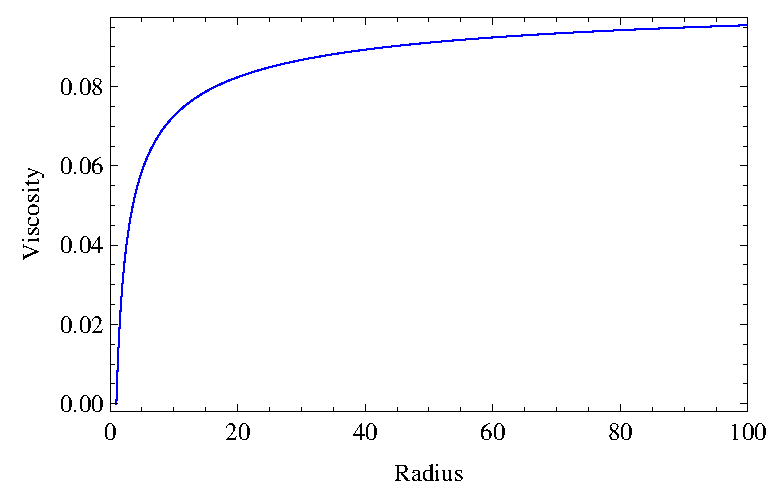
\includegraphics[width=3in]{viscosity.eps}
	\caption{This figure shows the shape of the relationship between viscosity and radius.  This plot was created using Eq. (\ref{massFlow}) with nonspecific values of other variables ($\dot{M} = \mu = R_* = 1$).  At radii near the star, the viscosity increases rapidly.  At further radii, it flattens out and approaches an asymptotic value. \label{viscosityFig}}
\end{figure}
\begin{figure} [b!]
	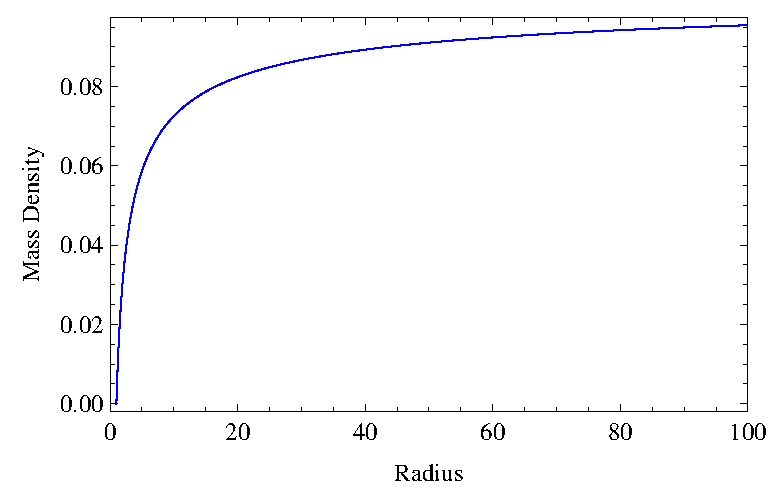
\includegraphics[width=3in]{massDensity.eps}
	\caption{This figure shows the shape of the relationship between mass density and radius.  This plot was created using Eq. (\ref{massFlow}) with nonspecific values of other variables ($\dot{M} = \nu = R_* = 1$).  Clearly, as evidenced by the parallelism of $\nu$ and $\mu$ in Eq. (\ref{massFlow}), this follows the same relationship described by Fig. \ref{viscosityFig}.  \label{massDensityFig}}
\end{figure}
Typical stars rotate less rapidly than the Keplerian velocity of the disk describes.  Thus,
\begin{equation}
\Omega_* < \Omega_K\bigg|_{R_*}
\end{equation}

Imagine that the dust of the protoplanetary disk extends radially inward to a far enough extent so as to be continuous up to the surface of the star.  This difference in angular velocity between the disk constituents and the star requires that angular momentum be lost when they fall into the star as a result of their radially inward drift velocity.  This requires a boundary layer of thickness $b$ in which the disk's material falls from the angular velocity of $\Omega_K$ to $\Omega_*$.  

Typically, $b \ll R_*$ and, therefore, $\Omega$ is extremely close to its typical Keplerian value where $\Omega' = 0$.  At this point,
\begin{equation}
\Omega(R_* + b) = \left(\frac{GM_*}{{R_*}^3} \right)^{1/2} \left[1 + X(b/R_*) \right], \label{nearStarOmega}
\end{equation}
where $X[b/R_*]$ is some small fraction.  In this regime, we must evaluate Eq. (\ref{modifiedAng1}), which takes on the form
\begin{equation}
C = 2\pi R_*^3 \mu u_r \Omega(R_* + b) , \nonumber
\end{equation}
around the point $R_* + b$.  Using the result of Eq. (\ref{nearStarOmega}), the constant, $C$,  is determined to be
\begin{equation}
C = - \dot{M}(G M R_*)^{1/2}. \nonumber
\end{equation}
Using this boundary condition-dependent constant along with Eq. (\ref{modifiedAng1}), we find that
\begin{equation}
\nu \mu = \frac{\dot{M}}{3\pi}\left[ 1 - \sqrt{\frac{R_*}{r}} \right], \label{massFlow}
\end{equation}
providing for us a governing equation of how mass would flow with respect to viscosity and surface density in a steady state disk.  How these variables vary with respect to radius is shown in Figs. (\ref{massFlowFig}), (\ref{viscosityFig}), \& (\ref{massDensityFig}).

\subsubsection{\label{section 2.2.2} Disk effective temperature}
Returning momentarily to our arbitrary ring of thickness $dr$, we must acknowledge that there are competing torques on the inner and outer edge of the ring, taking the form
\begin{equation}
\Gamma(r + dr) - \Gamma(r) = \frac{\partial \Gamma}{\partial r}dr \nonumber.
\end{equation}
As this torque is aligned with angular momentum, we can utilize the product rule of derivatives to find the rate at which this torque works on our disk, namely,
\begin{equation}
\Omega\Gamma(r + dr) - \Gamma(r) = \left[ \frac{\partial}{\partial r}(\Gamma\Omega) - \Gamma\Omega' \right]dr.
\end{equation}
The first of the right-hand terms corresponds to the 'convection' of rotational energy throughout the disk, whereas the $\Gamma\Omega' dr$ term corresponds to the rate at which mechanical energy is lost.  Due to the geometry of the disk, this energy must be radiated from the top and bottom surfaces, each of which has a surface area of approximately $(2\pi r)dr$. Dividing the dissipated energy by the total surface area from which it radiates, we find an expression for the disk's total viscous dissipation \cite{king2002},
\begin{equation}
D(r) = \frac{\Gamma \Omega'}{4\pi r}= \frac{1}{2}\nu \mu (r\Omega')^2,
\end{equation}
and substituting our findings in Eq. (\ref{massFlow}), we find that
\begin{equation}
D(r) =\frac{1}{2}\frac{\dot{M}}{3\pi}\left[ 1 - \sqrt{\frac{R_*}{r}} \right] (r\Omega')^2. \nonumber
\end{equation}
Setting $\Omega = \Omega_K$ and using
\begin{equation}
r\frac{\partial\Omega_K}{\partial r} = -\frac{3}{2}\sqrt{\frac{G M_*}{r^3}},
\end{equation}
we find that
\begin{equation}
D(r) = \frac{3GM_*\dot{M}}{8\pi r^3}\left[ 1 - \sqrt{\frac{R_*}{r}} \right].
\end{equation}

At this point we bring forth another assumption about the nature of these disks: that is, they are optically thick in the $z$-direction.  Accordingly, the disk radiates like a blackbody following the Stefan-Boltzmann law, which states that the energy flux of a body is proportional to the fourth power of absolute temperature,
\begin{equation}
E_{\text{flux}} = \sigma T^4,
\end{equation}
where $\sigma$ is the Stefan-Boltzmann constant.  For our disk system, we know that $E_\text{flux} = D(r)$, and as such, the temperature of the disk can be expressed such that \cite{armitage2011, king2002}
\begin{equation}
T(r) = \left( \frac{3GM_*\dot{M}}{8\pi r^3 \sigma}\left[ 1 - \left( \frac{R_*}{r}\right)^{1/2}\right] \right)^{1/4}. \label{tempEq}
\end{equation}
The variance of temperature with respect to radius is shown in Fig. \ref{tempFig}.


\subsection{\label{section2.3} Disk viscosity models}
\begin{figure} [t!]
	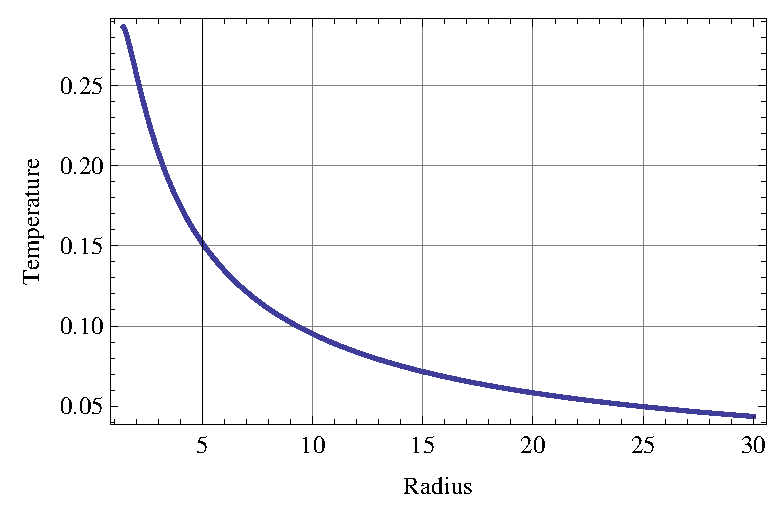
\includegraphics[width=3in]{temperature.eps}
	\caption{This figure shows how temperature of the disk varies with respect to radius, as described by Eq. (\ref{tempEq}), using non-specific values of $M_* = \dot{M} = \sigma = R_* = 1$.  As would be expected, the temperature of the disk is high near to the star, and falls off rapidly to a low asymptotic value as the radius increases. \label{tempFig}}
\end{figure}
While our current assumptions, namely that disk turbulence is local and that there are no external torques acting on the disk, have proven useful in finding the temperature profile of the disk, in order to say anything further it will be necessary to specify the disk's viscosity, $\nu$.  The classical approach at such a point is to assume that
\begin{equation}
\nu = \alpha \frac{c_s^2}{\Omega_K} = \alpha c_s h , \label{nuRelation}
\end{equation}
where $c_s$ is the speed of sound in the disk and the second equality follows from the assumption of vertical hydrostatic equilibrium (specifically, that $h \approx c_s/\Omega_D$.  In this equation, $\alpha$ is some dimensionless function which will remain constant if there is a simple scaling relation between $\nu$ and locally defined flows.  While exceptionally simple, the assumption of a constant $\alpha$ allows for the construction of a remarkably complete description of disk evolution.  Unfortunately, it is unlikely that such models of constant $\alpha$ pertain to protoplanetary disks; both the magnetic fields and the changing temperature gradient within the disks make it unlikely that the viscosity near the star is equal to that of the viscosity very far from the star \cite{armitage2011}.

Fortunately, there are a number of other methods in use for determining a value of $\alpha$.  For example, it is possible to determine a relationship for $\nu(r)$ if one has knowledge of $\mu$ and $\dot{M}$ within a disk, via Eq. (\ref{massFlow}).  Other methods for determining $\alpha$ or $\nu(r)$ are beyond the scope of this paper.

\subsubsection{\label{section 2.3.1} Simple-$\alpha$ models of protoplanetary disks}
While constant $\alpha$ models may not be perfectly appropriate for describing protoplanetary disks, that does not mean they are useless in efforts to understand disk dynamics, as one of the simplest methods of constructing computational models of protoplanetary disks is by assuming that $\alpha$ in Eq. (\ref{nuRelation}) is constant.  In such cases, disk structure becomes a function of $\Omega_D$, $\mu$, and our constant $\alpha$.  One significant prediction which has been made through the use of simple $\alpha$ models is that the surface density profile of a steady-state disk takes on the form $\mu \propto r^{-1}$.  Additionally, although not entirely accurate, simple $\alpha$ models provide a useful starting point for making estimates on how other important disk quantities should vary with respect to disk radius.  




\section{\label{section 3} Angular momentum transport via self-gravity}
It is a well-known fact that the self-gravity of a massive disk which is subject to radiative cooling results in angular momentum transport and accretion \cite{armitage2011}.  In a disk for which magnetism is unimportant, the stability of the disk can be quantified using gravitational effects, the centripetal force, and pressure through a quantity known as the Toomre $Q$ parameter.

\subsection{\label{section 3.1} Derivation of the Toomre $Q$ parameter}
Imagine, as we have been, a large, flat disc of radius R made up of constituent gases and particles with a large solar mass, $M_*$, at its center and some overall mass density $\mu_{\text{mean}}$ rotating with a roughly constant angular velocity, $\vec{\Omega}$. Suppose that for this disc, the centripetal acceleration at any point $\vec{r}$ is roughly equal to 
\begin{equation}
\vec{a}_{\text{cp}} = \left( \vec{\Omega} \times \vec{r} \right) \times \vec{\Omega} ,
\end{equation}
and suppose that this balances acceleration due to gravitation,
\begin{equation}
\vec{a}_{\text{g}} = -\frac{G M_*}{r^2}\hat{r}, 
\end{equation}
where $G$ is the universal gravitational constant.

\subsubsection{\label{section 3.1.1} The effects of disturbances on centripetal acceleration and gravitational acceleration}
Now suppose that a small square area of $L^2$ experiences a contraction such that the local mass density changes by a factor $\epsilon$.  In this space, $\mu_{\text{local}} = (1+\epsilon) \mu_{\text{disk}}$. This change also results in an equivalent contraction of the length dimension, such that $L_\text{local} = L/(1 + \epsilon)^{1/2}$. Particles at the border of such a region would experience a local change in gravitation,
\begin{multline}
\Delta a_{\text{g}} =(a_{\text{g-local}} - a_{\text{g-mean}}) \\
= \frac{G\mu_\text{disk} (1 + \epsilon) (L/(1 + \epsilon)^{1/2})^2}{L^2} - \frac{G\mu_{\text{disk}} L^2}{L^2}
\\
= G \mu_{\text{disk}}\left(\frac{1}{1 + \epsilon} - 1  \right) \nonumber
\end{multline}
Taking a Maclaurin series of $(1 + \epsilon)^{-1}$, we find that \cite{toomre1964}
\begin{equation}
\Delta F_\text{g} \approx G\mu_\text{disk}\epsilon
\end{equation}

Around such a region, there would also be a change in particles' local angular velocities.  That is, with respect to the center of the compressed region, the particles would experience a change in local angular velocity on the order of 
\begin{equation}
\Delta \Omega_\text{local}^2 = \left(\frac{u_\text{orb}}{L/(1+\epsilon)^{1/2}}\right)^2 - \left(\frac{u_\text{orb}}{L}\right)^2 =  \epsilon\Omega_\text{local}^2.
\end{equation}
As a result, any particle bordering this region in the outward radial direction would experience a change in local centripetal force of \cite{toomre1964}
\begin{equation}
\Delta (\Omega_\text{local}^2 L) = \epsilon \Omega_\text{local}^2 L
\end{equation}

If we balance out these two disturbances, we find that 
\begin{equation}
G \mu_\text{disk} \epsilon = \epsilon \Omega_\text{local}^2 L.
\end{equation}
It is clear that the change in centripetal acceleration cannot overcome the former change in gravitational force below some critical length, $L_\text{crit}$, where
\begin{equation}
L_\text{crit} \approx \frac{G \mu_\text{disk}}{\Omega_\text{local}^2}. \label{crit1.1}
\end{equation}
In order to gain an appreciation for the order of magnitude of these disturbances must take, we recall that for a stable disk,
\begin{equation}
\Omega^2 R \approx \frac{G\mu_\text{mean} R^2}{R^2} = G\mu_\text{disk},
\end{equation}
where $\mu_\text{mean}$ is the mean mass density of the disk.  Substituting this result into Eq. (\ref{crit1.1}), we find that
\begin{equation}
L_\text{crit} \approx \left(\frac{\mu_\text{disk}}{\mu_\text{mean}}\right)\left(\frac{\Omega}{\Omega_\text{local}}\right)^2 R,
\end{equation}
informing us that disturbances required to cause such gravitational instability must be on the order of magnitude of the radius of the disk itself \cite{toomre1964}.

\subsubsection{\label{section 3.1.2} The effects on random motion on instability}
For any disk in stable rotation, we know that
\begin{equation}
\Omega_\text{local}^2 R = \frac{u_{\phi}^2}{L} = G \mu_\text{disk}. \label{stableDiskBalance}
\end{equation}
One necessary criterion for stability is that two particles, traveling through a compressed region of length $L$ such as that described in the previous section, must travel with respect to one another a distance roughly as large as the instability in a time during which the stability would have grown.  This time can be expressed in terms of the velocities of the particles, such that 
\begin{equation}
t_\text{motion} = \frac{L}{u_\phi}.
\end{equation}
Solving for $u_\phi$ in Eq. (\ref{stableDiskBalance}), we find that
\begin{equation}
t_\text{motion} = \sqrt{\frac{L}{G\mu_\text{disk}}}.
\end{equation}

We must now simplify our model for a moment, from a rotating disc to a sheet of particles each with some mean-square random velocity of $\langle u^2 \rangle$. Clearly in such a case, the time required to cross a disturbance of size $L$ is
\begin{equation}
t_\text{rand} = \frac{L}{\langle u^2 \rangle^{1/2}}.
\end{equation}
Although this result is derived from an exceptionally simplified case, it will be a useful approximation in the case of a rotating disk.  Using this insight along with the time of evolution of an instability in a rotating disk, we find that the disk is stable only when the time required for non-random motions to pass through the region of instability is greater than the time of instability of random motions, such that
\begin{equation}
t_\text{motion} > t_\text{rand}.
\end{equation}
As a result, we find a second critical length depended upon average motion of particles, where average motions are only capable of keeping a region stable with a length below or roughly equal to
\begin{equation}
L_u \approx \frac{\langle u^2 \rangle}{G\mu_\text{disk}}. \label{crit2.1}
\end{equation}

\subsubsection{\label{section 3.1.3} The Toomre $Q$ parameter}
Combining the results of Eqs. (\ref{crit1.1}) \& (\ref{crit2.1}), we know that the disk is stable only where $L_u > L_\text{crit}$, or where
\begin{equation}
\frac{\langle u^2 \rangle}{G\mu_\text{disk}} > \frac{G \mu_\text{disk}}{\Omega_\text{local}^2} \nonumber
\end{equation}
Rearranging, we find a parameter relating to gravitational stability, where \cite{whittle2010}
\begin{equation}
\frac{\langle u^2 \rangle^{1/2} \Omega_\text{local}}{G\mu_\text{disk}} > 1.
\end{equation}
At this point, it is important to recognize that our local angular rotation, which is often known as ``local vorticity'' is often expressed using one of Oort's constants \cite{whittle2010}, where
\begin{equation}
\Omega_{local} = \nabla \times \vec{u} = B = -\frac{1}{2}r\left(\frac{d\Omega}{dr} + \frac{2\Omega}{R}  \right)_{R_*}
\end{equation}
We can also express $B$ in terms of the epicyclic frequency of rotation of the disk, $\kappa$, where \cite{whittle2010}
\begin{equation}
\kappa^2 = -4B\Omega.
\end{equation}
As $\kappa/\Omega \approx 4/\pi$, we can approximate $B$, and therefore $\Omega_\text{local}$, as
\begin{equation}
B = \Omega_\text{local} = \frac{\kappa}{\pi}
\end{equation}
Renaming our random motion $\langle u^2 \rangle ^{1/2}$ as the stellar velocity dispersion, $\sigma$, our equation becomes
\begin{equation}
Q = \frac{\sigma \kappa}{\pi G\mu_\text{disk}} > 1, \label{qParam}
\end{equation}
where $Q$ is called the Toomre $Q$ parameter and specifies the necessary conditions for the gravitational stability of a disk.  From this parameter, it is clear to see that low velocity dispersion, low local rotation, low epicyclic frequencies and/or exceptionally high mass density favor gravitational instability \cite{whittle2010}.  Relationship of this parameter with respect to $\sigma$, $\kappa$, and $\mu_\text{disk}$ is shown in Fig. \ref{qFig}.

\begin{figure} [b!]
	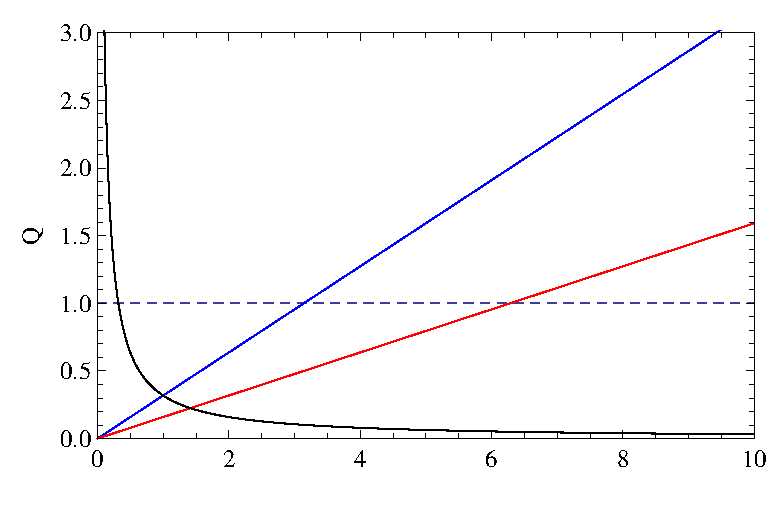
\includegraphics[width=3in]{qplot.eps}
	\caption{This figure shows how the Toomre $Q$ parameter changes with respect to $\sigma, \kappa,$ or $\mu_\text{disk}$ when all other variables are held constant.  The blue line shows how the parameter changes with respect to $\sigma$ when $\kappa = \mu_\text{disk} = 1$, the red shows how the parameter changes with respect to $\kappa$ when $2\sigma = \mu_\text{disk} = 1$, and the black line shows how it changes with respect to $\mu_\text{disk}$ when $\sigma = \kappa = 1$.  Values of $Q > 1$ allow for gravitational stability, whereas values of $Q \lesssim 1$ show gravitational instability.  Clearly gravitational stability favors high values of $\kappa$ and $\sigma$ and low values of $\mu_\text{disk}$. \label{qFig}}
\end{figure}



\subsection{\label{section 3.2} Effects of gravitational Instability}
Gravitational instability is typically a seen in young protoplanetary disks which are massive and have large radii.  Once a disk is gravitationally unstable, numerical simulations have determined three possible outcomes of disk evolution.  It is possible for the disk to setting into a quasi-steady, "saturated" state in which there is a large amount of sel-gravitating turbulence and trailing spiral arms allow for outward motion of angular momentum.  A second possibility finds the disk exhibiting large accretion bursts.  A third, and more interesting possibility, shows the disk fragmenting into distinct bound objects, which can be crucial in planet formation or in the formation of large stellar objects \cite{armitage2011}.

\subsection{\label{section 3.3} Gravitational Instability and planet formation}
Theoretically, there are two conditions required for gravitational fragmentation to occur.  First, for the disk in which fragmentation occurs, we must find that $Q \lesssim 1$.  However, in addition to that, it is necessary for the proto-fragment to cool at a sufficiently rapid pace for energy delivered via compression to be radiated away.  Simulations have shown disks successfully achieving gravitational instability at around 30 AU when radiation from the central star is not accounted for.  Unfortunately, those simulations show strong spiral arms developing but no tendency to fragment gravitationally, as the disk is incapable of radiating energy at a rapid enough pace.  On the other hand, those simulations which have included the central star's radiation show a disk with the capability of radiating a sufficient quantity of energy, but such disks show no inclination of gravitational instability at small radii \cite{whitworth2007}.

That being said, it has been shown that Sun-like stars occasionally form with massive, extended protoplanetary disks.  In such cases, brown dwarfs, planetary mass objects, or low-mass Hydrogen-burning stars are likely to form via gravitational instability at the far reaches of the disk.  When brown dwarfs do form from fragmentation, they are often liberated from the inner star's gravitational pull, often removing a significant portion of the accretion disk around the original star to form a stable accretion disk around the young, free brown dwarf.  In fact, a single protoplanetary disk of this sort is capable of creating a large number of brown dwarfs by itself.  these liberated stars will often eventually find a similarly liberated companion and form double brown dwarf binary systems with low mass ratios \cite{hubber2007}.  



\section{\label{section 4} Further Topics}
While this paper has set up a framework for examining the dynamics and gravitational stability of protoplanetary disks, there are a number of significant topics in disk evolution which were outside of the scope of this summary.  For example, while simple $\alpha$ models of viscosity are useful, there is a large amount of literature on the derivation and effects of more complicated models of $\alpha$.  Additionally, although here we examined self-gravity and gravitational instability, it is clear that this is but one of many important topics involved in disk development and fragmentation.  Two particularly notable topics which were outside of the scope of this paper were disk radiation and magnetorotational instability.  For a brief overview of all relevant topics in disk evolution, I refer the reader to ``Dynamics of Protoplanetary Disks'' \cite{armitage2011}.

\bibliography{Bibliography}

\end{document}